\section{Proof Walkthrough}\label{sec:walkthrough}

\begin{enumerate}
  \item Initial state
  \\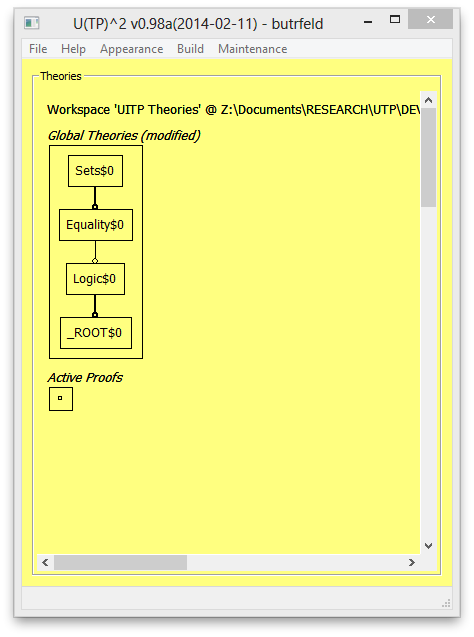
\includegraphics[scale=0.5]{SCREENSHOTS/01-initial-state.png}
  \item Set axioms
  \\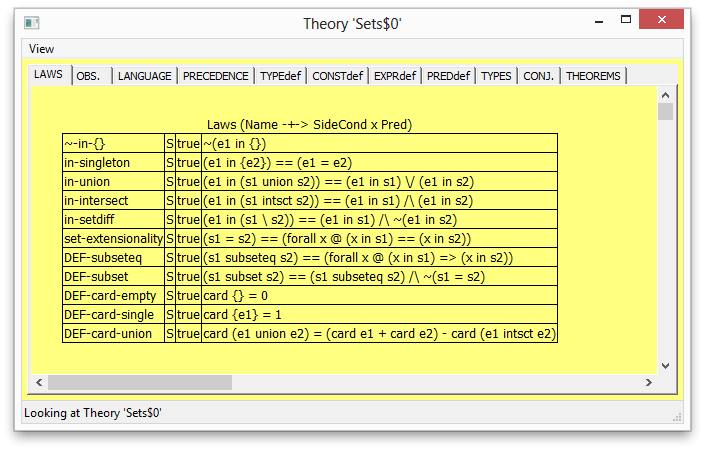
\includegraphics[scale=0.5]{SCREENSHOTS/02-set-axioms.png}
  \newpage
  \item Set Conjectures
  \\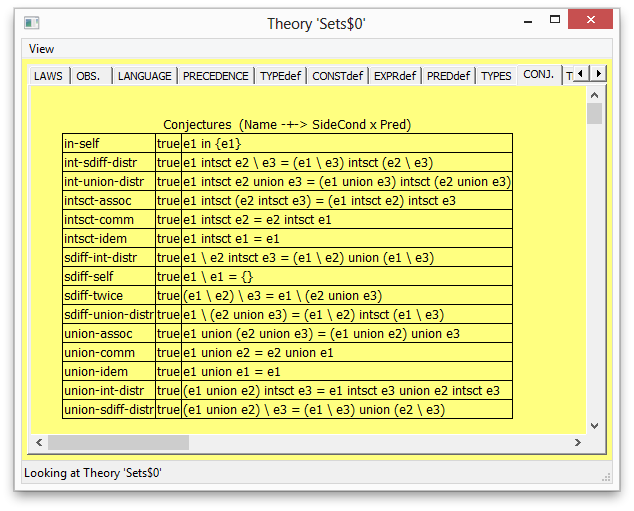
\includegraphics[scale=0.5]{SCREENSHOTS/03-set-conjectures.png}
  \item Starting Proof
  \\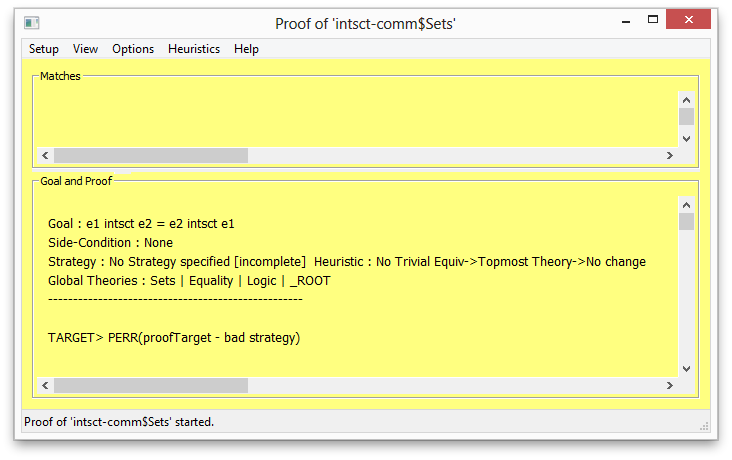
\includegraphics[scale=0.5]{SCREENSHOTS/04-starting-proof.png}
  \newpage
  \item Proof Setup menu
  \\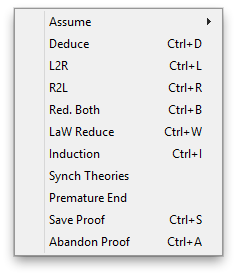
\includegraphics[scale=0.5]{SCREENSHOTS/05-proof-setup-menu.png}
  \item Starting REDUCE Proof
  \\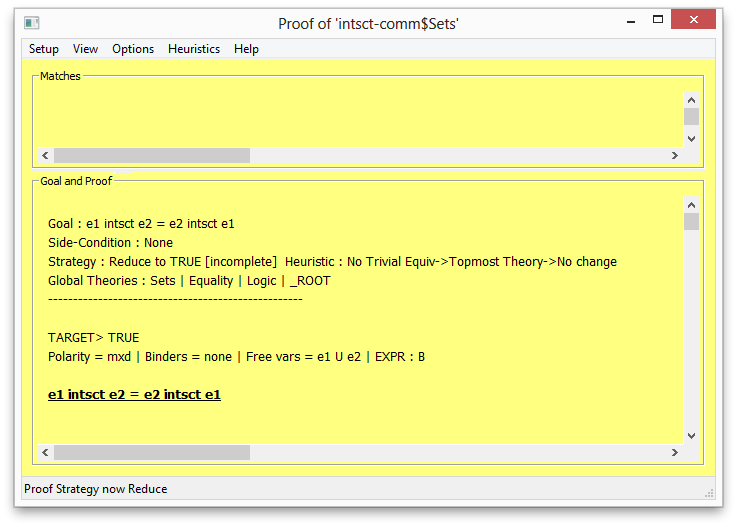
\includegraphics[scale=0.5]{SCREENSHOTS/06-starting-REDUCE-proof.png}
  \newpage
  \item Laws Applicable to top goal
  \\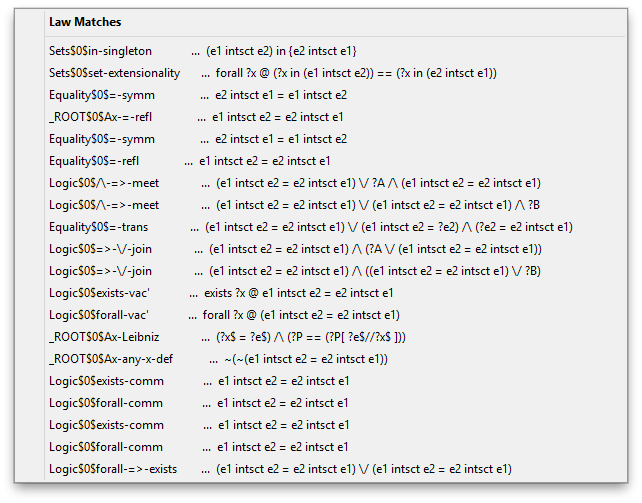
\includegraphics[scale=0.5]{SCREENSHOTS/07-laws-applicable-to-goal.png}
  \item Instantiating Bound Variables
  \\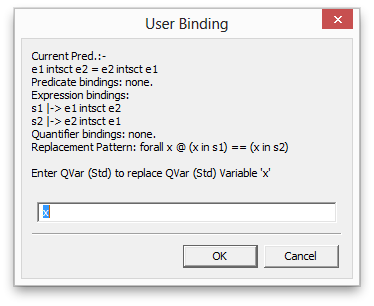
\includegraphics[scale=0.5]{SCREENSHOTS/08-instantiating-qvars.png}
  \newpage
  \item Applying Set Extensionality
  \\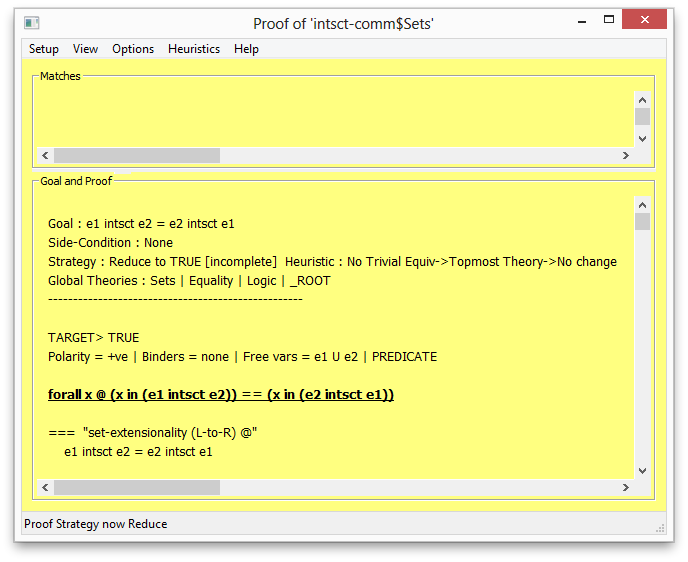
\includegraphics[scale=0.5]{SCREENSHOTS/09-extensionality-applied.png}
  \item Moving Down (down-arrow)
  \\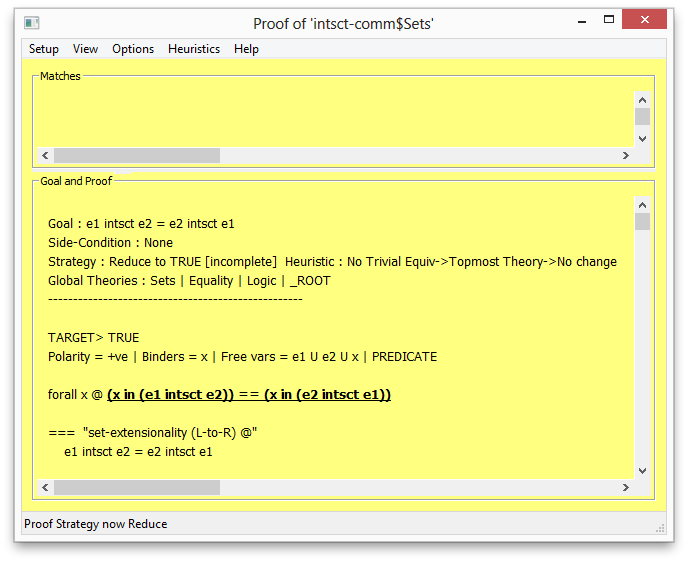
\includegraphics[scale=0.5]{SCREENSHOTS/10-moving-down.png}
  \newpage
  \item Moving Down again (down-arrow)
  \\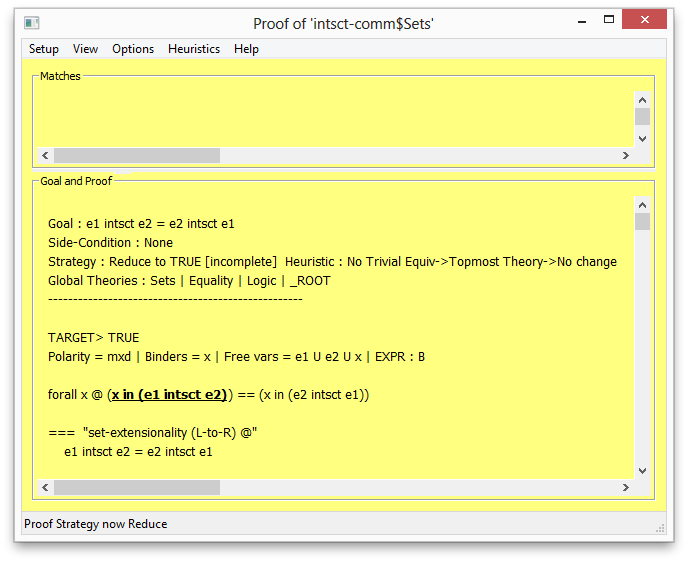
\includegraphics[scale=0.5]{SCREENSHOTS/11-moving-down-again.png}
  \item Laws applicable to current focus
  \\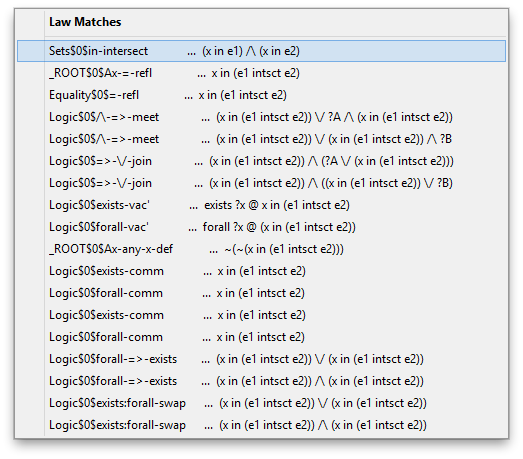
\includegraphics[scale=0.5]{SCREENSHOTS/12-laws-applicable-to-focus.png}
  \newpage
  \item Applying intersection axiom.
  \\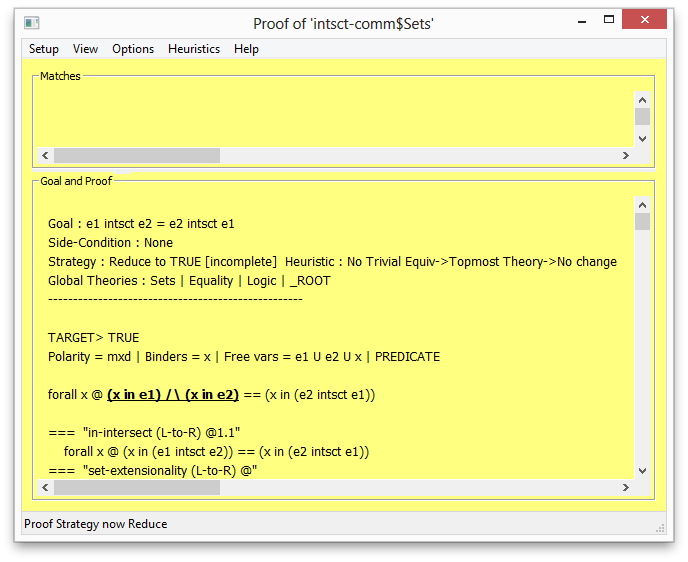
\includegraphics[scale=0.5]{SCREENSHOTS/13-intersect-axiom-applied.png}
  \item Applying commutativity
  \\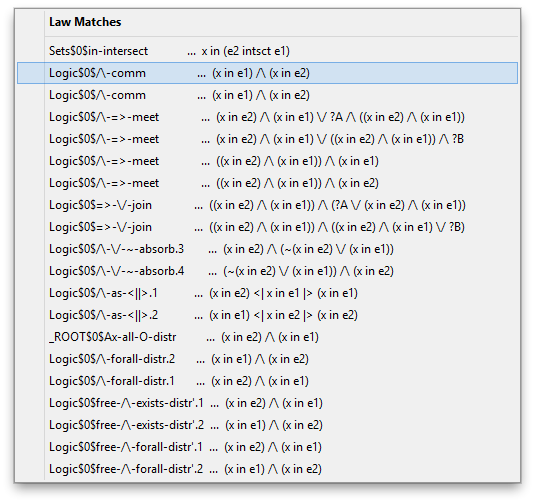
\includegraphics[scale=0.5]{SCREENSHOTS/14-applying-commutativity.png}
  \newpage
  \item Apply Reflexivity of Equality
  \\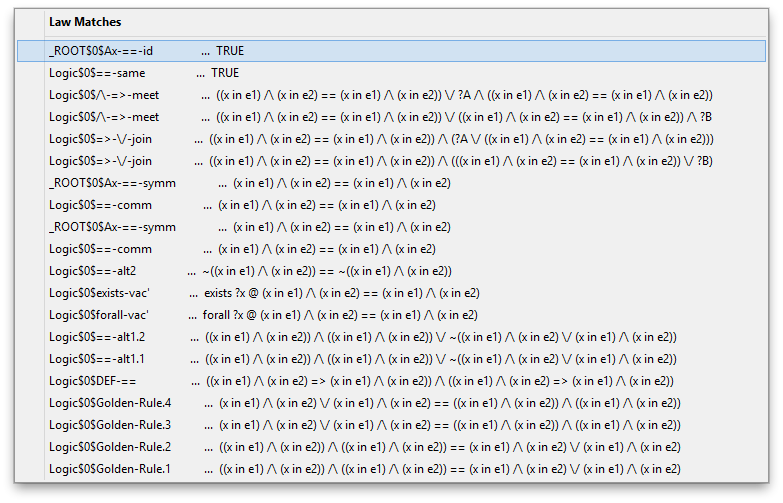
\includegraphics[scale=0.5]{SCREENSHOTS/15-applying-equal-reflexive.png}
  \item Eliminating Vacuous quantifier
  \\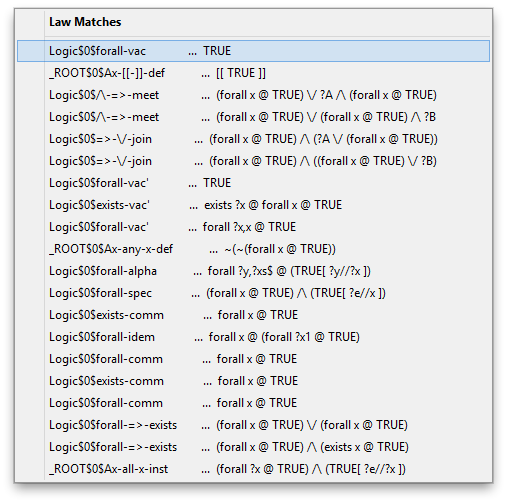
\includegraphics[scale=0.5]{SCREENSHOTS/16-vacuous-quantifier.png}
  \newpage
  \item Proof now complete
  \\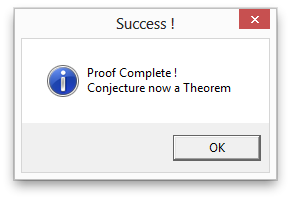
\includegraphics[scale=0.5]{SCREENSHOTS/17-proof-complete.png}
  \item Finished Proof
  \\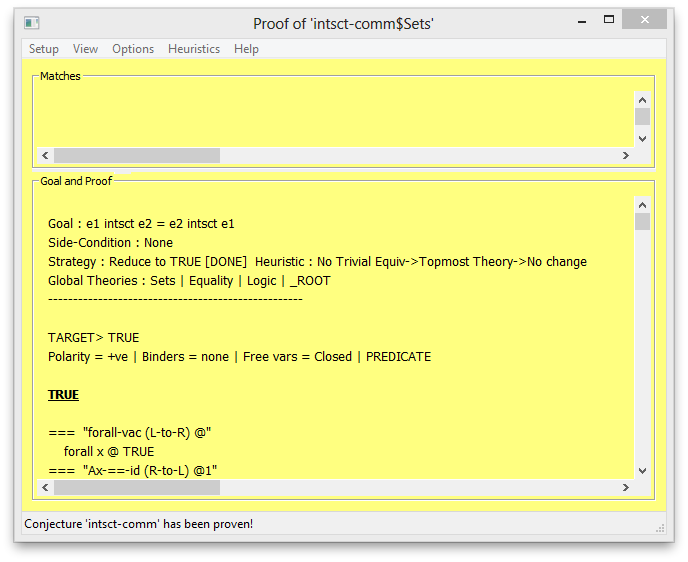
\includegraphics[scale=0.5]{SCREENSHOTS/18-finished-proof.png}
  \newpage
  \item New Theorem added into Law pool.
  \\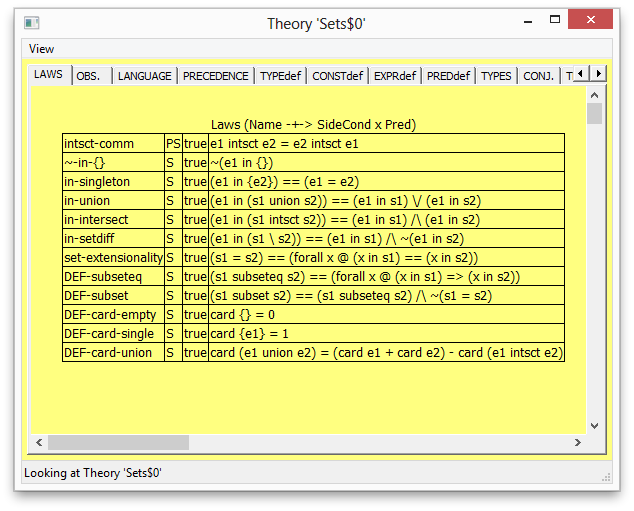
\includegraphics[scale=0.5]{SCREENSHOTS/19-laws-with-new-theorem-added.png}
  \item The new Theorem
  \\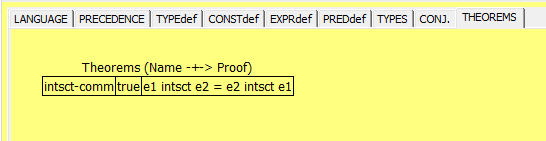
\includegraphics[scale=0.5]{SCREENSHOTS/20-our-new-theorem.png}
  \item Saving a Text Version
  \\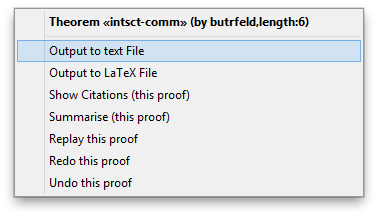
\includegraphics[scale=0.5]{SCREENSHOTS/21-saving-text-version.png}
  \newpage
  \item Final State
  \\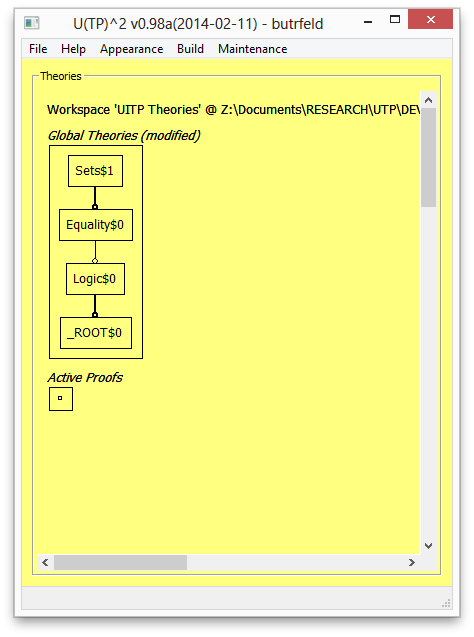
\includegraphics[scale=0.5]{SCREENSHOTS/22-final-state.png}
  \end{enumerate}

The proof text:
\begin{verbatim}
Complete Proof for 'Sets$intsct-comm
Goal : e1 intsct e2 = e2 intsct e1
Strategy: Reduce to TRUE

     e1 intsct e2 = e2 intsct e1
 ===   " set-extensionality (L-to-R) @ "
     forall x @ (x in (e1 intsct e2)) == (x in (e2 intsct e1))
 ===   " in-intersect (L-to-R) @1.1 "
     forall x @ (x in e1) /\ (x in e2) == (x in (e2 intsct e1))
 ===   " in-intersect (L-to-R) @1.2 "
     forall x @ (x in e1) /\ (x in e2) == (x in e2) /\ (x in e1)
 ===   " /\-comm (R-to-L) @1.2 "
     forall x @ (x in e1) /\ (x in e2) == (x in e1) /\ (x in e2)
 ===   " Ax-==-id (R-to-L) @1 "
     forall x @ TRUE
 ===   " forall-vac (L-to-R) @ "
     TRUE
\end{verbatim}
